\subsection{Results and Analysis}

\begin{todolist}
\item mention a table that includes the number of qubits/layer/random parameter for each ansatz
\item describe more in figure \ref{Variance Local Cost}
\item analysis instead of describe
\item add the figures above (python notebook) for analysis
\item describe how alternating data leads to different result(s).
\end{todolist}

The section \ref{Development Process section} dicusses the configurations of the experiment. 
We summarize the experiment results as the table:
\begin{center}
    \begin{tabular}{|| c c c ||}
        \hline
        Ansatz      & Method                                & Variance of gradients \\[0.5ex] 
        \hline \hline
        NLocal      & None                                  & Decay                 \\
        \hline
        TwoLocal    & None                                  & Decay                 \\
        \hline
        NLocal      & Local Cost Function, Shallow circuit  & Sustain               \\
        \hline
        TwoLocal    & Local Cost Function, Shallow circuit  & Sustain               \\
        \hline
    \end{tabular}
\end{center}

For the default setting, the two ansatzes' gradient variances decay as expected.
As the number of qubits scales up, the variances decay exponentially, this indecates that the cost function landscape becomes flatter and flatter. 
We suspect that the result would be inefficientcy for any gradient-based optimization algorithm to train the model.
We discussed this phenomenon in Section \ref{Barren Plateaus section}.
Figure \ref{Plot ansatzes gradients default} shows the results of the two ansatzes in this configuration.

\begin{figure}
    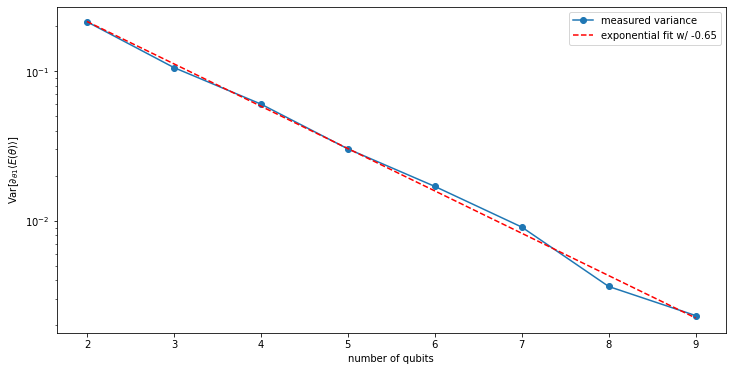
\includegraphics[width=\textwidth]{Artefact/Appendices/NLocalDefault.png}
    \centerline{a) NLocal Ansatz gradient variance values}
    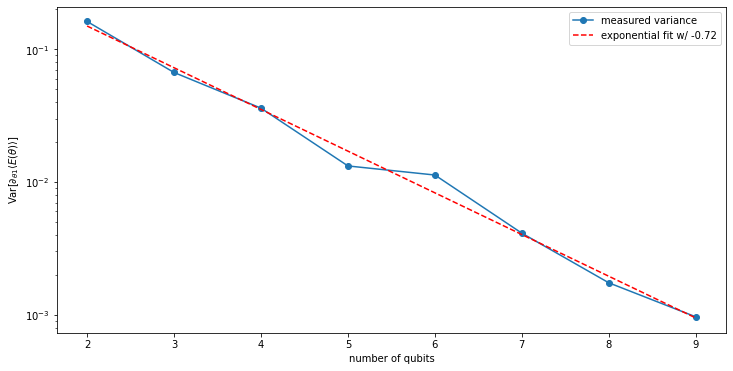
\includegraphics[width=\textwidth]{Artefact/Appendices/TwoLocalDefault.png}
    \centerline{b) TwoLocal Ansatz gradient variance values}
    \caption{
        The variances of gradient from differences ansatzes.
        On both plots: the variances vanish exponentially to the number of qubits, ansatzes are in default configuration.
    }
    \label{Plot ansatzes gradients default}
\end{figure}

In contrast, for the case of Local Cost Function and Shallow circuit, we observe that the variances of the ansatzes' gradient did not vanished when we attempt to increase the number of qubits.
This implies that the cost function landscape can sustain the slope.
Figure \ref{Variance Local Cost} shows the result of the experiment for Local Cost Function and Shallow circuit, in comparison with the default settings.

\begin{figure}
    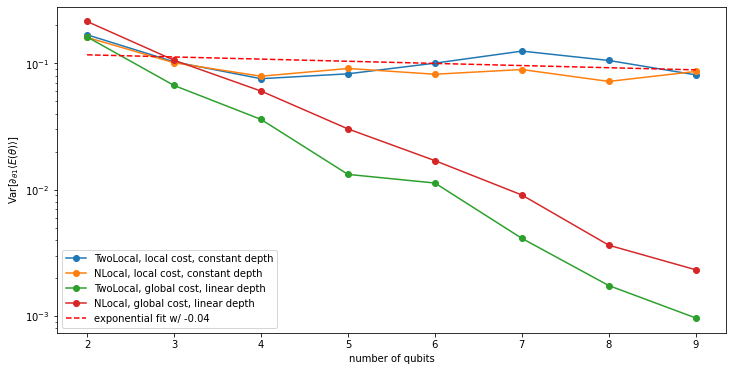
\includegraphics[width=\textwidth]{Artefact/Appendices/variancesLCF.png}
    \caption{
        Comparison of the variance values of the two ansatzes with and without Local Cost Function and constant depth.
        The ansatzes with Global Cost Function and increased depth have their gradient variances decay exponentially with the number of qubits. 
    }
    \label{Variance Local Cost}
\end{figure}
